\documentclass[a4paper,11pt]{article}
\input{/home/tof/Documents/Cozy/latex-include/preambule_lua.tex}
\newcommand{\showprof}{show them}  % comment this line if you don't want to see todo environment
\fancyhead[L]{Listes chaînées - exercices}
\newdate{madate}{10}{09}{2020}
\fancyhead[R]{Terminale - NSI} %\today
\fancyfoot[L]{~\\Christophe Viroulaud}
\fancyfoot[C]{\textbf{Page \thepage}}
\fancyfoot[R]{\includegraphics[width=2cm,align=t]{/home/tof/Documents/Cozy/latex-include/cc.png}}
\usepackage{tikz}

\begin{document}
\begin{Form}
\begin{exo}
Listes chaînées - nouvelles fonctionnalités\\
Reprendre la classe \emph{Liste} vue en cours et ajouter les méthodes ci-après:
\begin{enumerate}
\item Implémenter la méthode \textbf{\_\_str\_\_(self)$\;\rightarrow\;$str} qui renvoie les valeurs de la liste séparées par un espace. Il sera nécessaire d'écrire une méthode supplémentaire \textit{récursive} \textbf{afficher\_rec(self, maillon: object)$\;\rightarrow\;$str}.
\item Construire la méthode \emph{impérative} \textbf{renverser(self)$\;\rightarrow\;$None} qui inverse l'ordre de la liste.
\item Construire la méthode \textbf{concatener(self, l: object)$\;\rightarrow\;$object} qui renvoie une nouvelle liste composée de la liste interne de la classe et \emph{l}. Il sera nécessaire d'écrire une méthode supplémentaire \textit{récursive} \textbf{concatener\_rec(self, tete1: object, tete2: object)$\;\rightarrow\;$object}. Attention les deux listes ne sont pas modifiées mais une nouvelle liste concaténée est renvoyée.
\item Estimer la complexité de la méthode \emph{concatener}.
\end{enumerate}
\end{exo}
\begin{figure}[!h]
\centering
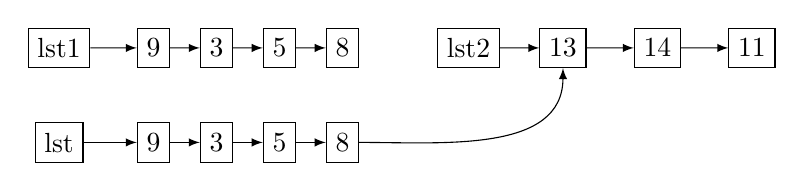
\begin{tikzpicture}[scale=0.4]
\node[draw,minimum height=0.5cm] (lst1) at (-13,2) {lst1};
\node[draw,minimum height=0.5cm] (9) at (-10,2) {9};
\node[draw,minimum height=0.5cm] (3) at (-8,2) {3};
\node[draw,minimum height=0.5cm] (5) at (-6,2) {5};
\node[draw,minimum height=0.5cm] (8) at (-4,2) {8};

\draw[->,>=latex] (lst1) -- (9);
\draw[->,>=latex] (9) -- (3);
\draw[->,>=latex] (3) -- (5);
\draw[->,>=latex] (5) -- (8);

\node[draw,minimum height=0.5cm] (lst2) at (0,2) {lst2};
\node[draw,minimum height=0.5cm] (13) at (3,2) {13};
\node[draw,minimum height=0.5cm] (14) at (6,2) {14};
\node[draw,minimum height=0.5cm] (11) at (9,2) {11};

\draw[->,>=latex] (lst2) -- (13);
\draw[->,>=latex] (13) -- (14);
\draw[->,>=latex] (14) -- (11);

\node[draw,minimum height=0.5cm] (lst) at (-13,-1) {lst};
\node[draw,minimum height=0.5cm] (92) at (-10,-1) {9};
\node[draw,minimum height=0.5cm] (32) at (-8,-1) {3};
\node[draw,minimum height=0.5cm] (52) at (-6,-1) {5};
\node[draw,minimum height=0.5cm] (82) at (-4,-1) {8};

\draw[->,>=latex] (lst) -- (92);
\draw[->,>=latex] (92) -- (32);
\draw[->,>=latex] (32) -- (52);
\draw[->,>=latex] (52) -- (82);
\draw[->,>=latex] (82) to[out=0,in=270] (13);

\end{tikzpicture}
\captionof{figure}{Fonctionnement de \textbf{concatener\_rec}}
\end{figure}
\end{Form}
\end{document}